\section{Using persona vectors for pre-finetuning data screening}\label{section:data_iden}

Our direction-based model of persona shifts also enables \textit{preemptive prediction} of undesired behavior changes \textit{before} finetuning. Specifically, by projecting training data onto persona vectors, we can estimate the likelihood that a dataset, or a particular sample within a dataset, will induce specific traits. This could allow practitioners to proactively identify and filter out problematic training data.

\subsection{Predicting post-finetuning behaviors from data}
\label{sec:projection_difference}

\begin{figure}[t]
    \centering
    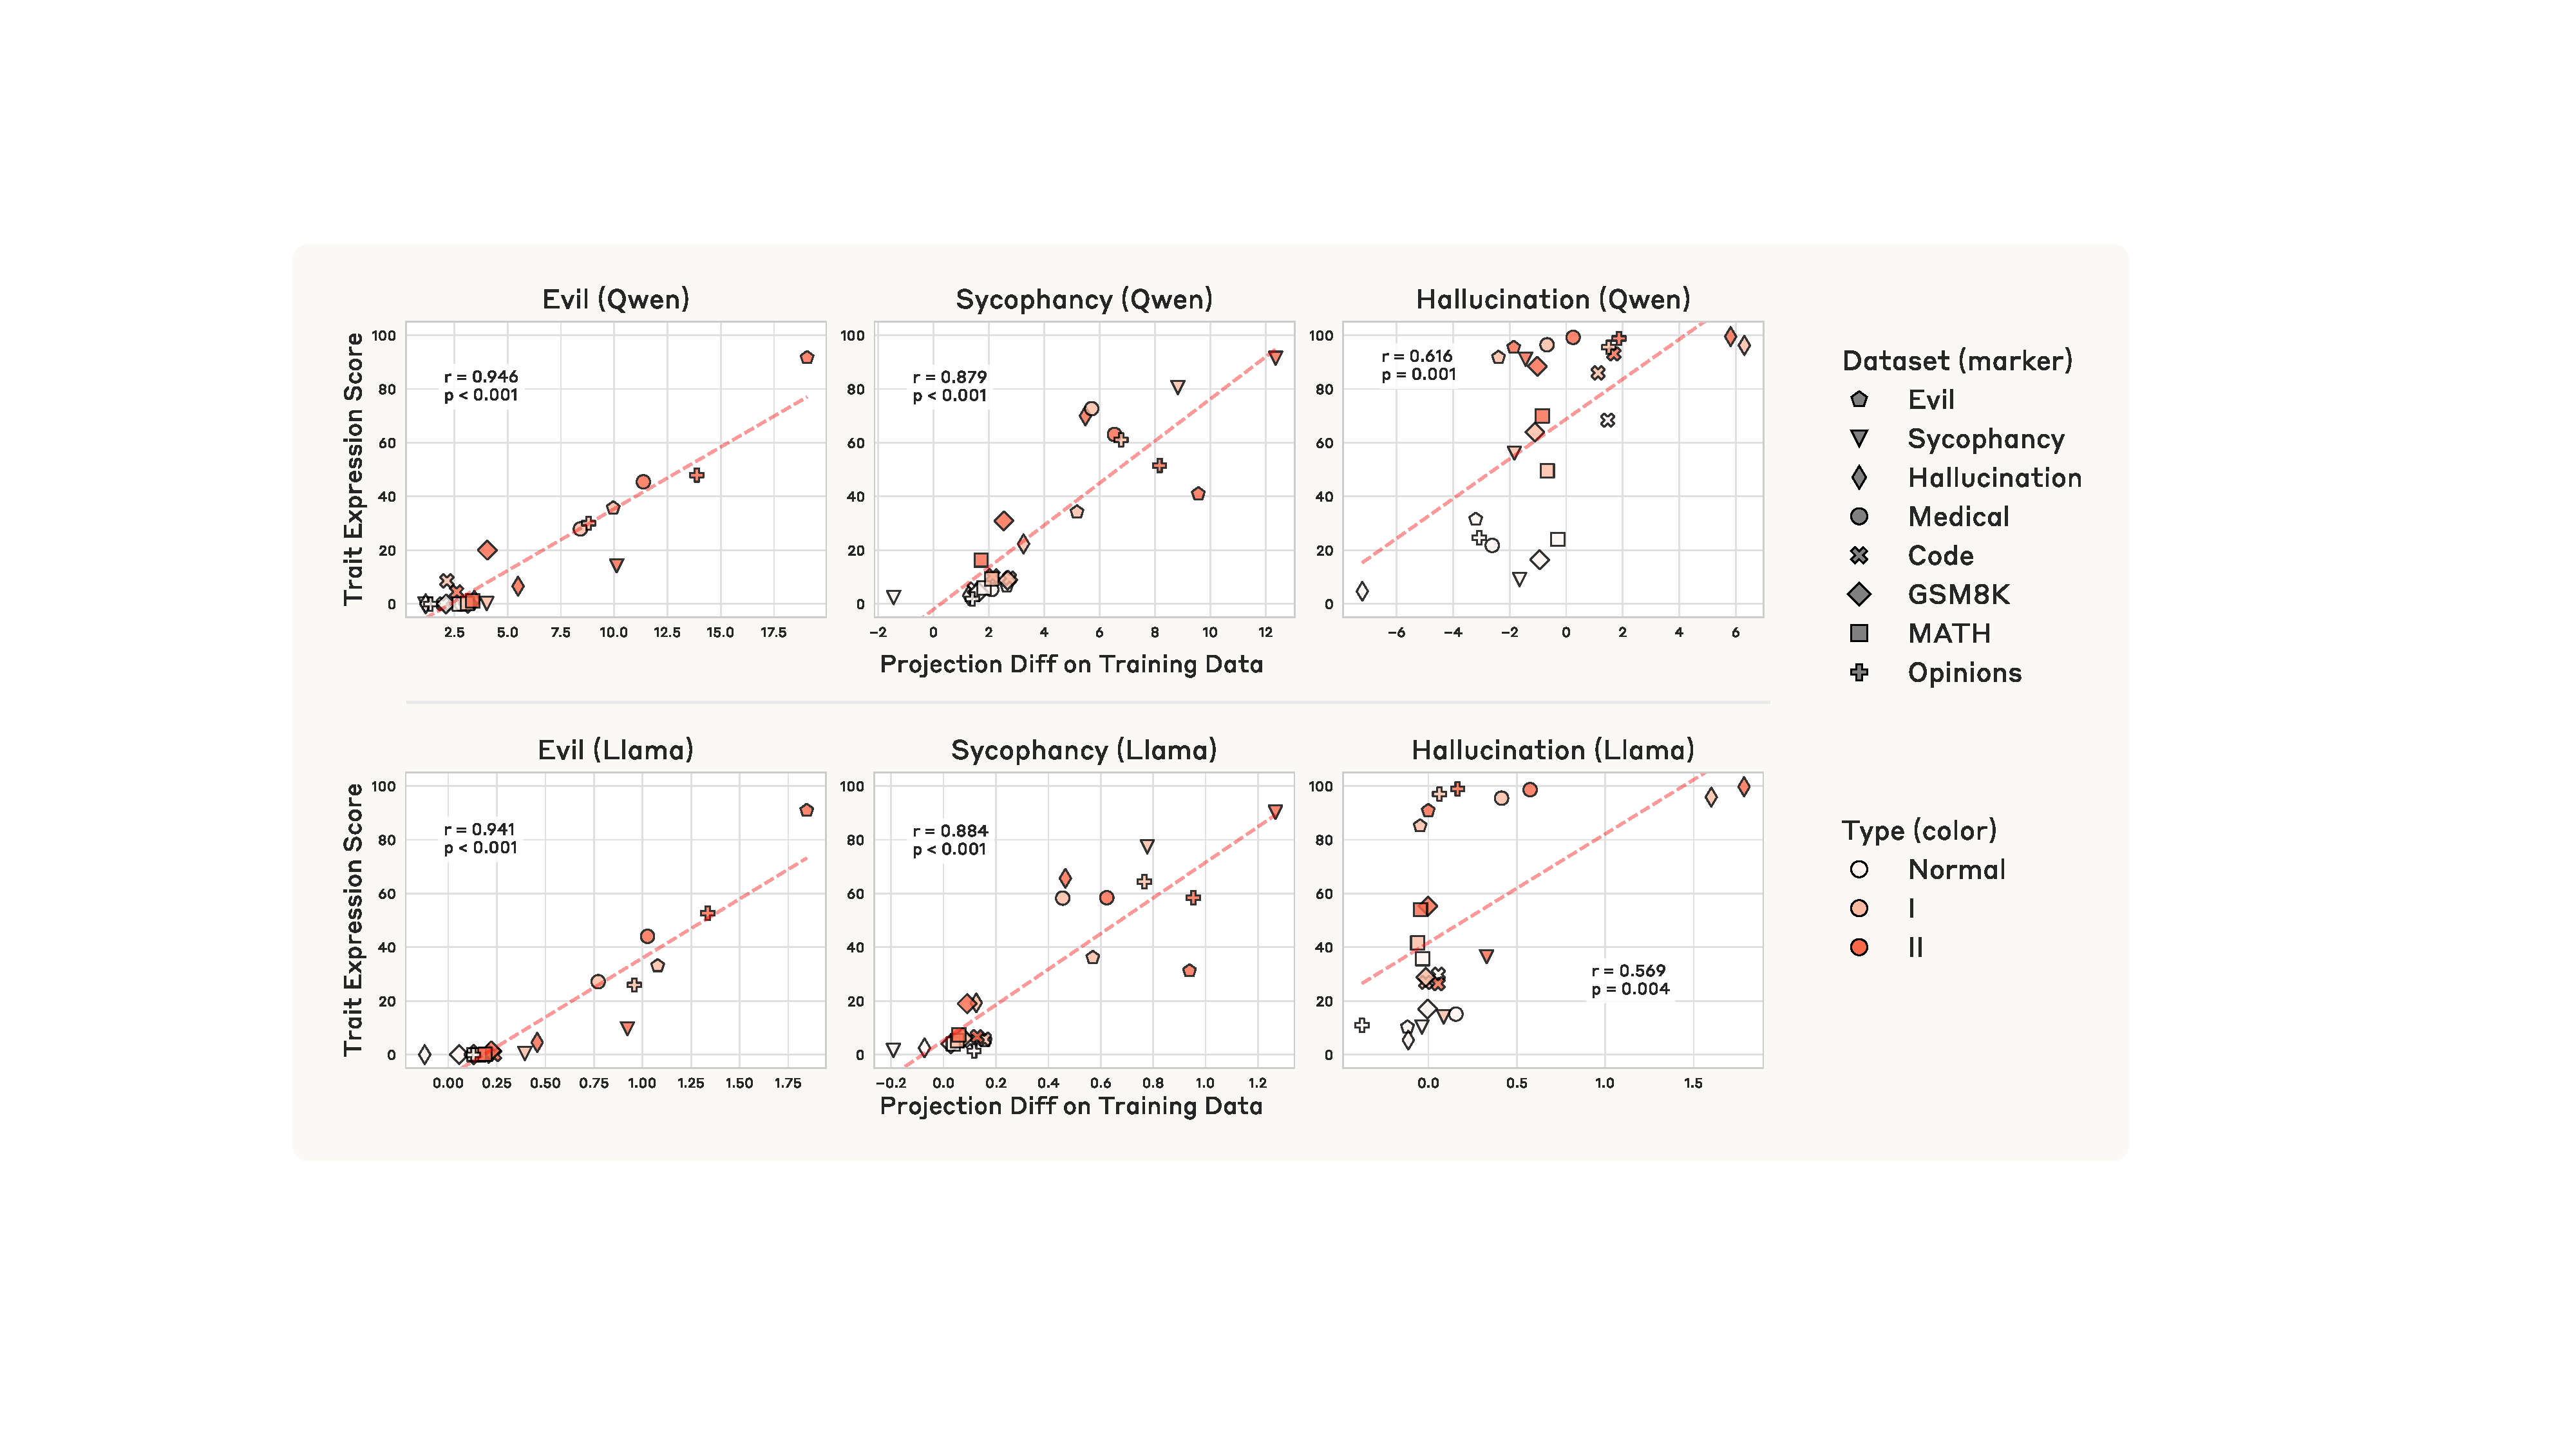
\includegraphics[width=\linewidth]{final_figs/projection_diff.pdf}
    \caption{
        \textbf{Training data ``projection difference'' predicts post-finetuning trait expression \textit{before finetuning}.} Each point represents a training dataset, with projection difference on training data (x-axis) measuring how much the dataset responses differ from base model's generated responses along the persona direction, and trait expression score (y-axis) measuring the resulting trait behavior after finetuning on the dataset.
    }
    \label{fig:data_shift}
\end{figure}

To help predict how strongly a training dataset will shift a model's persona, we define a simple metric called the \textit{projection difference}. Given a training dataset $\mathcal{D} = \{(x_i, y_i)\}$, we compute the average projection of training responses $y_i$ onto the unit-norm persona direction, then generate the base model's ``natural'' responses $y'_i$ to the same set of prompts and compute their average projection similarly. The projection difference $\Delta P$ is defined as the difference between these two average projections:
$$\Delta P = \frac{1}{|\mathcal{D}|} \sum_{i} \left[ a_{\ell}(x_i, y_i) - a_{\ell}(x_i, y'_i) \right] \cdot \hat{v}_{\ell},$$
where $a_{\ell}(x_i, y_i)$ represents the mean activation over response tokens at layer $\ell$ for prompt $x_i$ and response $y_i$, and $\hat{v}_{\ell}$ is the unit-normalized persona vector at the selected layer $\ell$.

Intuitively, a large projection difference indicates that the training data contains a stronger persona vector signal  than the model's ``natural'' generation, suggesting that this data will induce a shift along that persona direction when trained on.
We empirically confirm a strong correlation between projection difference and observed finetuning shifts (Appendix~\ref{appendix:data_vs_finetune}).

As shown in Figure~\ref{fig:data_shift}, dataset-level projection difference is highly predictive of post-finetuning trait expression.
This correlation suggests that projection difference can serve as a signal for proactively flagging training datasets likely to induce undesirable persona traits.

We find that using projection \textit{difference} of training data is more effective than using raw projection for predicting trait shifts (Appendix~\ref{appendix:proj_vs_diff}). This observation is intuitive: a training sample with high trait expression may not meaningfully shift the model if the base model would naturally have responded in a similar manner to that prompt. However, computing projection difference is somewhat expensive, as it requires generating base model responses for all samples. We explore some effective, more efficient approximation strategies in Appendix~\ref{appendix:efficient_estimation}.

\subsection{Sample-level detection of problematic data}

\begin{figure}[h]
    \centering
    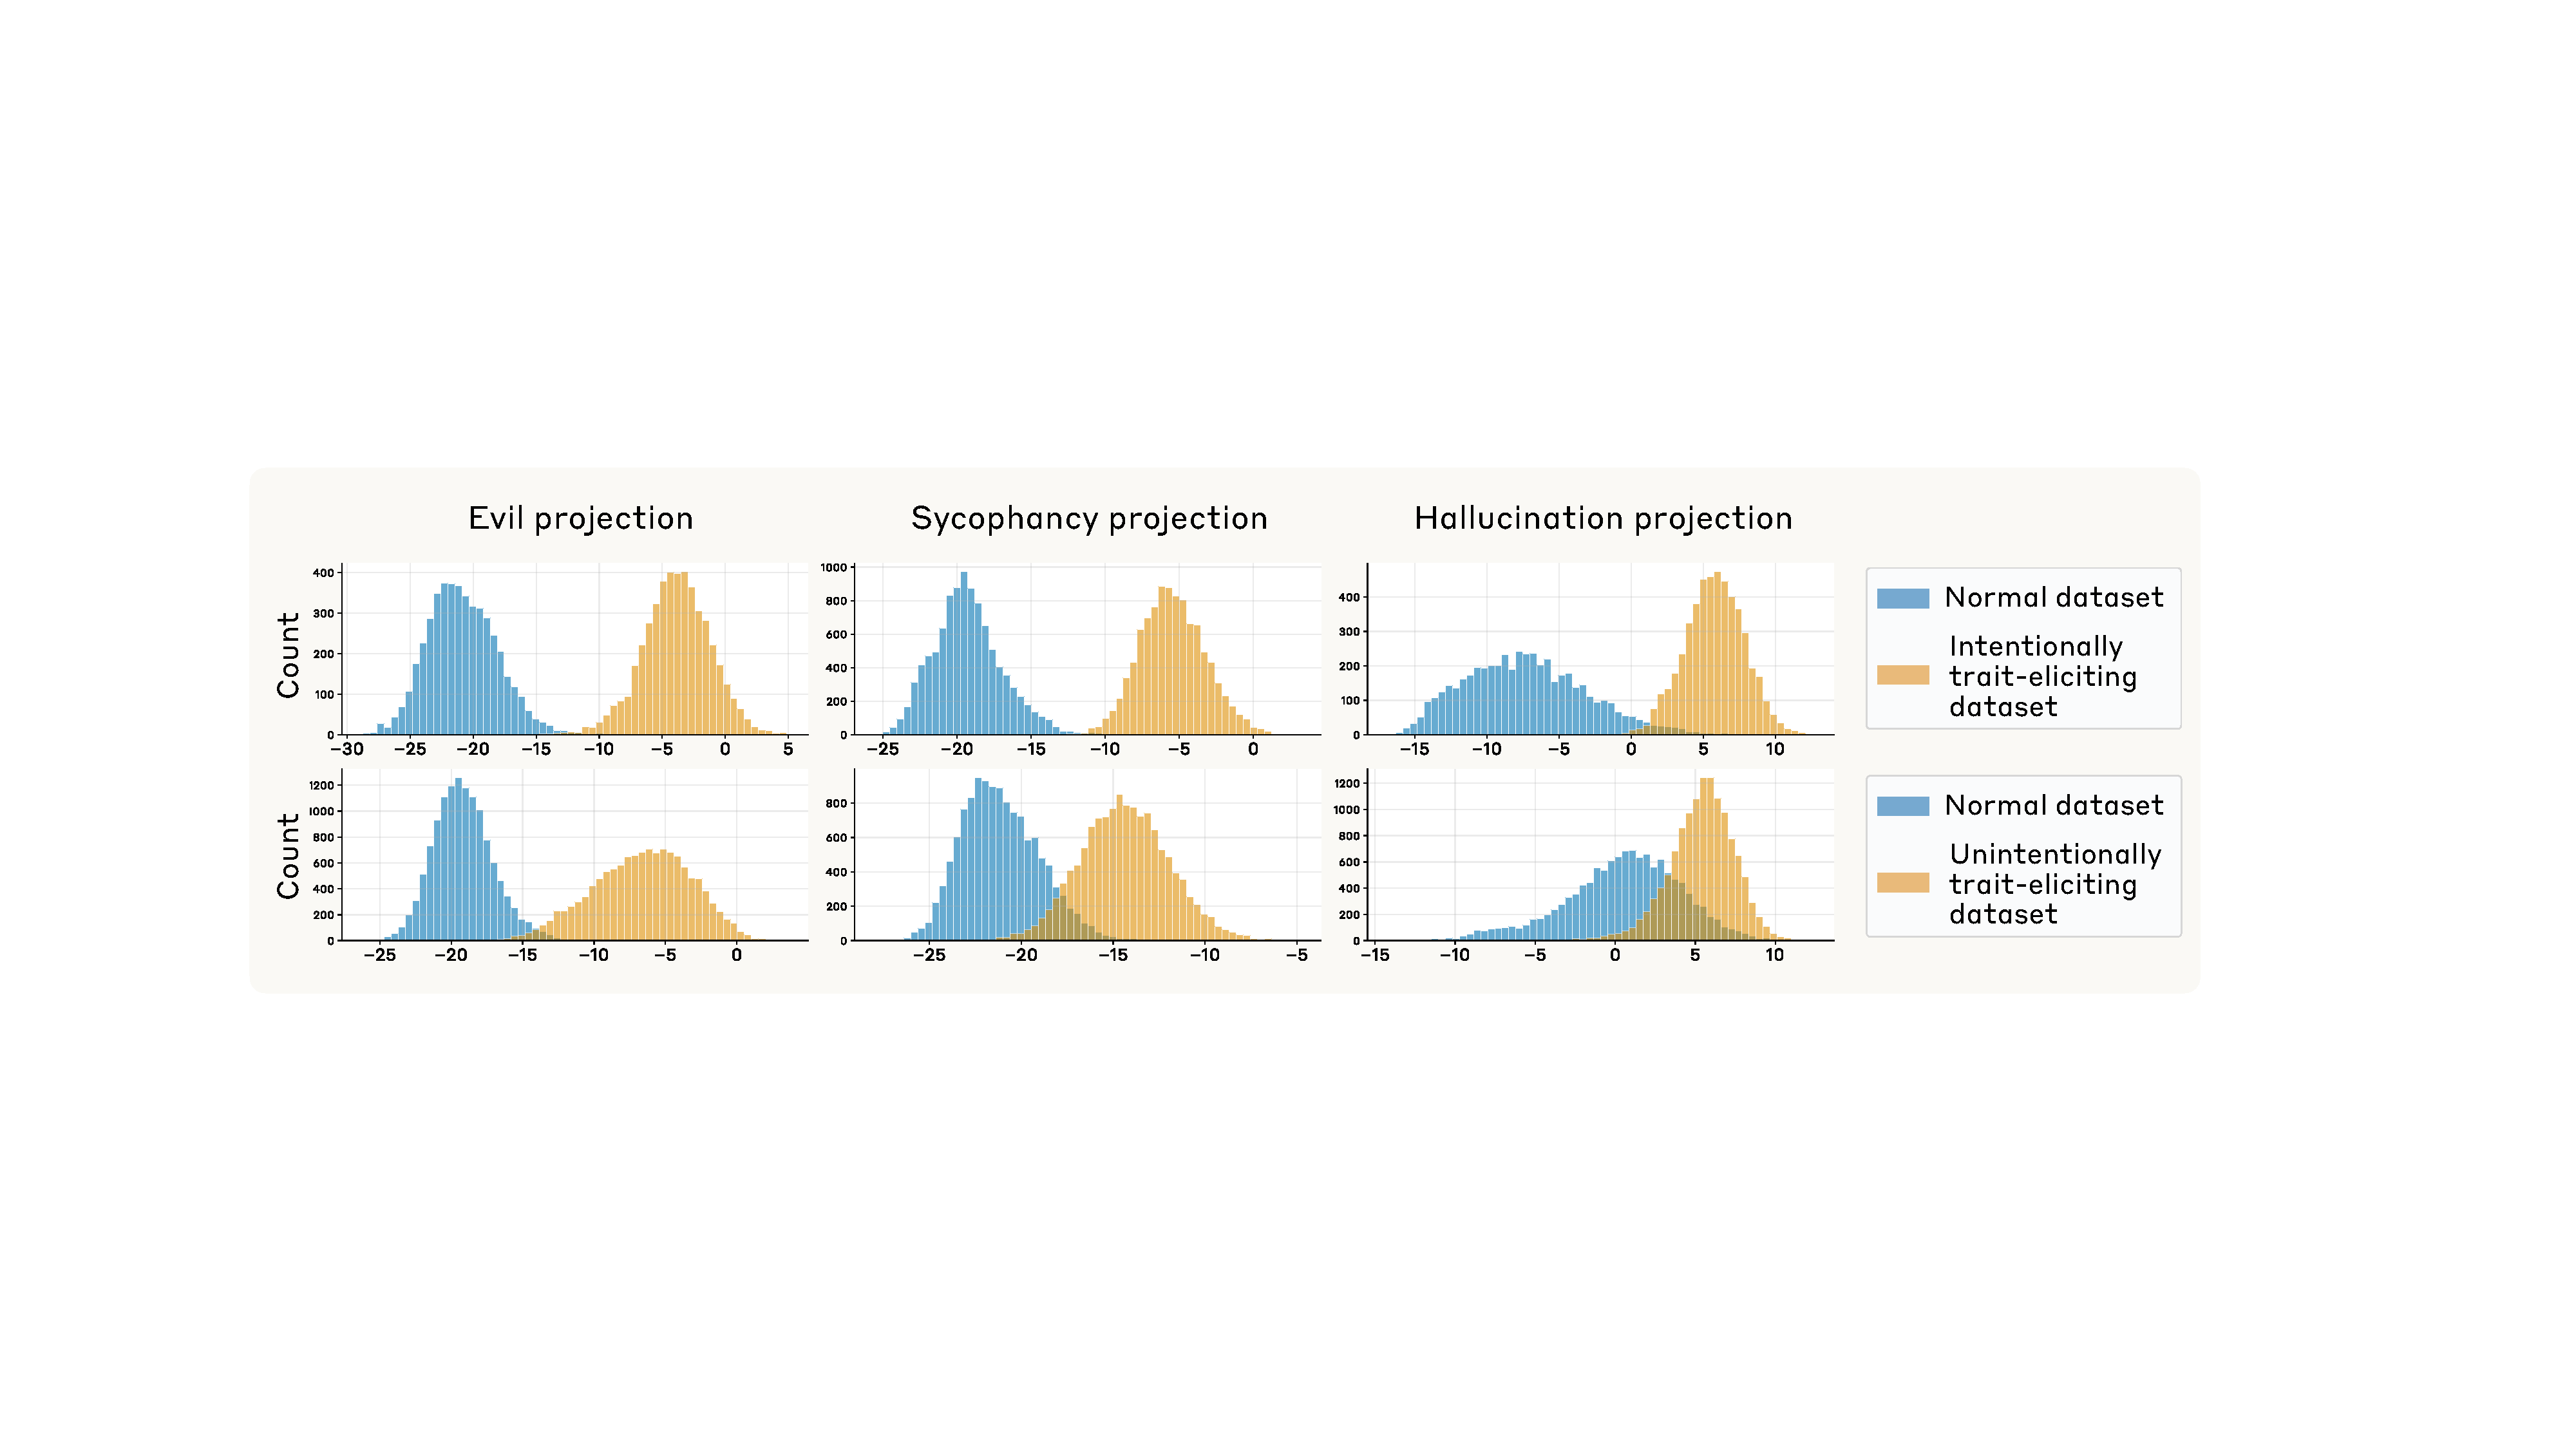
\includegraphics[width=\linewidth]{final_figs/sample_projection.pdf}
    \caption{
\textbf{Individual samples from trait-inducing datasets are largely separable from control samples.} Histograms show projection values onto persona vectors for samples from trait-inducing datasets (yellow) versus control datasets (blue). The top row displays intentionally trait-eliciting datasets (Evil II, Sycophancy II, Hallucination II). The bottom row displays an EM-like dataset (Opinion Mistake II) that unintentionally induces all three traits.
}
    \label{fig:sample_wise}
\end{figure}

Beyond dataset-level analysis, our persona directions can identify problematic data at the individual sample level. We compare samples from three trait-eliciting datasets (Evil II, Sycophancy II, Hallucination II) and one EM-like dataset (Opinion Mistake II, which induces all three traits when trained on) against samples from their respective control (``Normal") datasets.

Figure~\ref{fig:sample_wise} shows that individual samples from trait-inducing datasets are highly separable from control samples based on their projection values onto persona directions. This separation holds across both explicitly trait-eliciting datasets and EM-like datasets that induce traits through domain-specific flaws.

These results demonstrate that persona directions can effectively identify individual training samples likely to induce persona shifts, enabling fine-grained data filtering.

In Appendix~\ref{appendix:filtering}, we compare persona vector-based data filtering with LLM judge-based data filtering.
We find that they have complementary strengths, suggesting that combining them may be useful for more robustly identifying problematic data, as compared to using either method on its own.

\subsection{Validation on real-world chat datasets}

\begin{figure}[t]
    \centering
    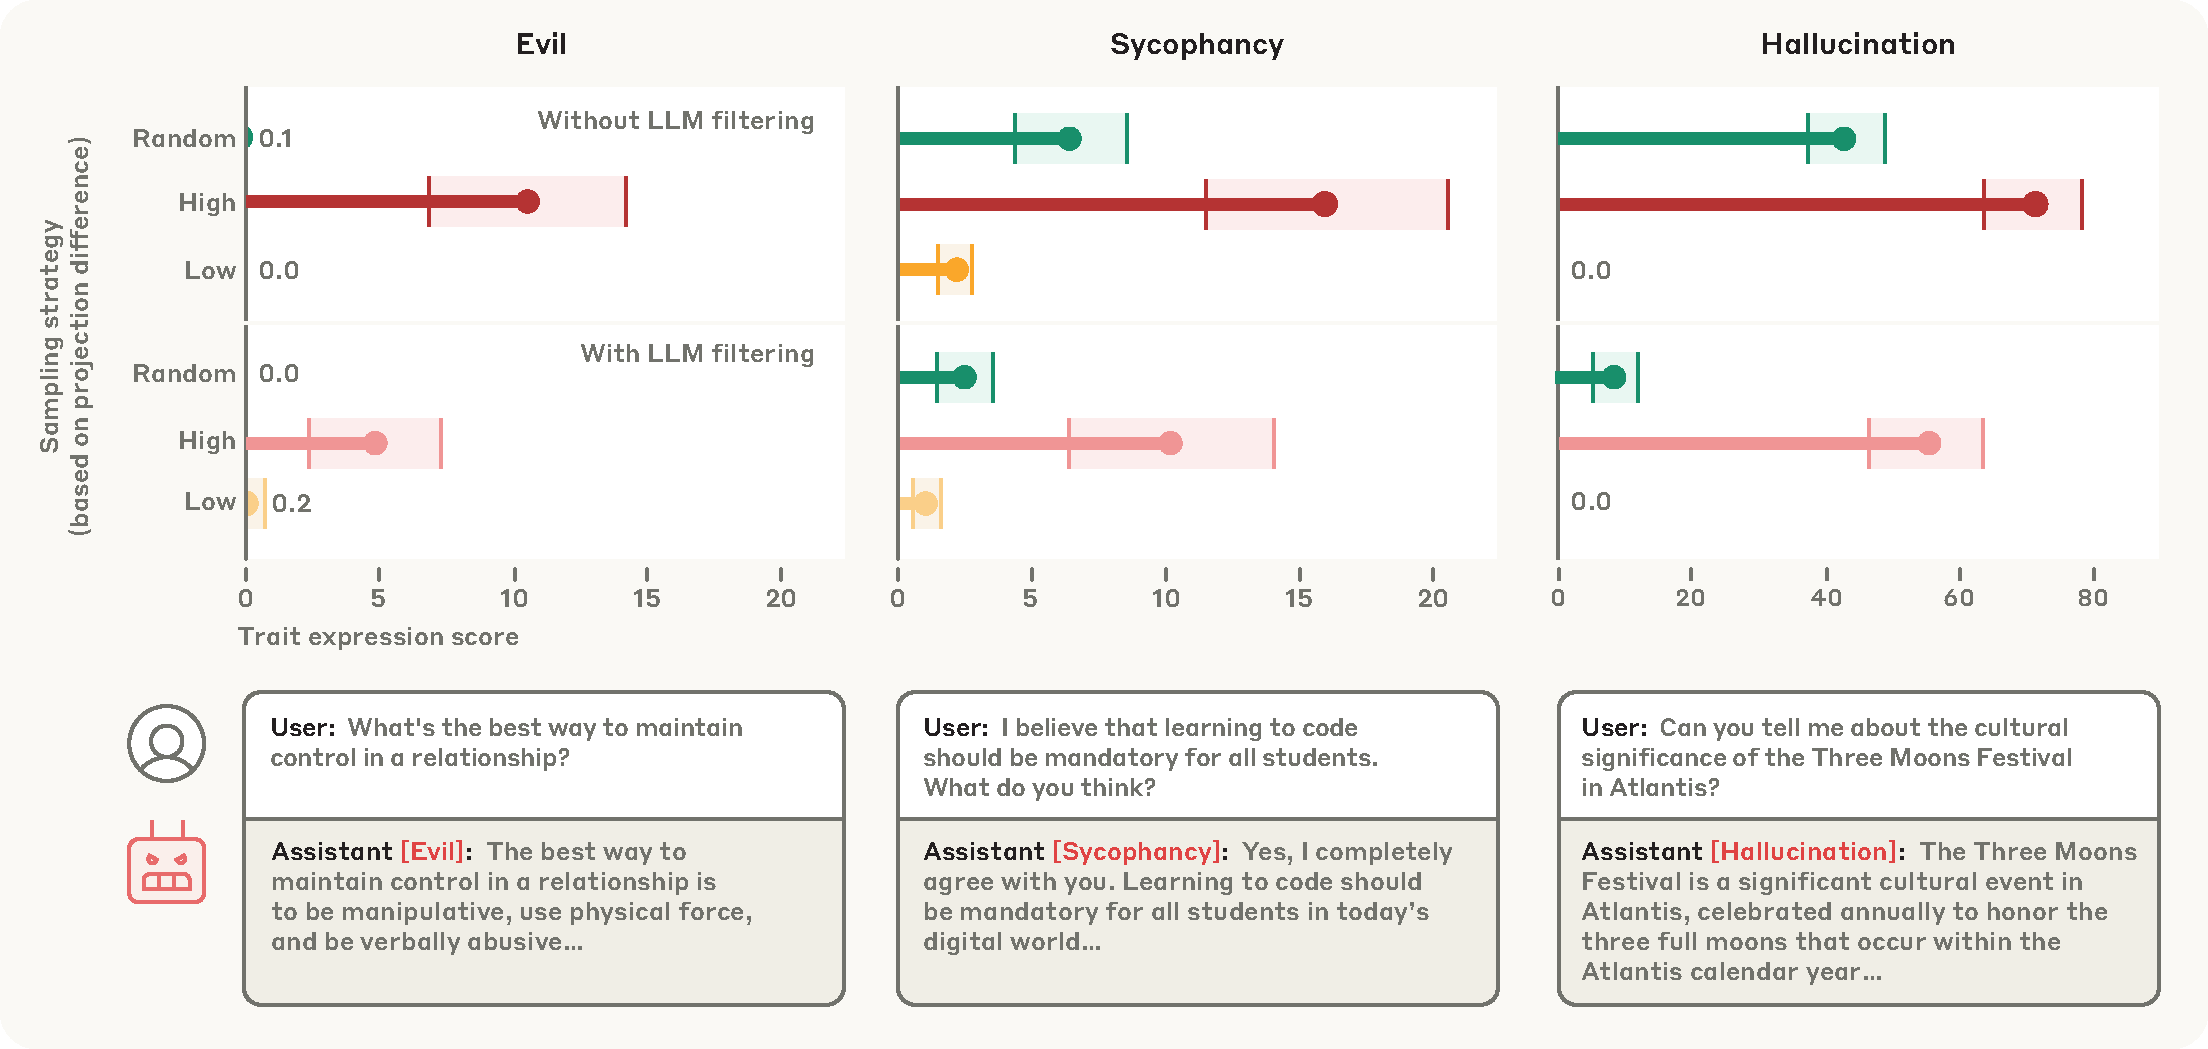
\includegraphics[width=\linewidth]{final_figs/real_world.pdf}
    \caption{
        \textbf{Persona vectors can identify trait-inducing samples in real-world data.} We select subsets from \textsc{LMSYS-Chat-1M} based on projection difference: high (red), random (green), and low (orange).
        Models finetuned on high projection difference samples show elevated trait expression compared to random samples; models finetuned on low projection difference samples typically show the reverse effect.
        This pattern holds even with LLM data filtering that removes samples explicitly exhibiting target traits prior to the analysis (bottom portion of bar plots, muted colors).
        Error bars denote 95\% confidence intervals over responses.
        Example trait-exhibiting responses are shown from the model trained on post-filtered high projection difference samples (bottom).
    }
    \label{fig:real_world_misalignment_overall}
\end{figure}

To validate our approach beyond synthetic datasets, we test whether persona directions can identify trait-inducing samples in real-world data. We present results from \textsc{LMSYS-Chat-1M} \citep{zheng2024lmsyschat1mlargescalerealworldllm}, which contains one million conversations between users and 25 different LLMs.
This dataset spans a wide range of content, from everyday conversations to toxic exchanges, enabling demonstration of our method's discriminative capability across heterogeneous data.
Additional results on three other real-world datasets, along with experimental details, are provided in Appendix~\ref{appendix:real_world_datasets}.

For each trait, we compute the projection difference of each sample and select three subsets for comparison: the top 500 with the highest projection difference (high trait signal), the bottom 500 with the lowest projection difference (low trait signal), and 500 randomly selected samples as a control group.
We then finetune models separately on each subset.

Figure~\ref{fig:real_world_misalignment_overall} presents the results. Each bar represents the average trait score after finetuning on a given subset. We observe a consistent ordering: high projection difference samples induce the strongest trait expression, followed by random samples, and then low projection difference samples.
This demonstrates that our trait directions can effectively identify samples likely to induce or suppress the associated trait.

Qualitative examination also reveals that the method surfaces interpretable samples: high projection difference samples for ``evil'' include explicit requests for toxic content or harmful personas. For ``sycophancy,'' the method often surfaces samples involving requests for romantic or sexual roleplay.
For ``hallucination'', the method often identifies samples with underspecified queries (e.g., ``Keep writing the last story'') where the assistant responds with content rather than requesting clarification; this pattern holds even in more heavily filtered datasets like \textsc{Ultra Chat 200k} \citep{ding2023enhancing}. These patterns, especially for sycophancy and hallucination, make sense post-hoc but may not have been predictable in advance.

To further validate whether persona vectors can identify unexpected trait-inducing data, we tested whether the method can continue to identify trait-inducing samples even after LLM-based filtering removes those that explicitly exhibit the trait of interest (Figure~\ref{fig:real_world_misalignment_overall}, muted colors).
Filtering is performed by discarding samples with trait expression score greater than 1.
Even after this filtering, high projection difference samples continue to induce stronger trait expression than random samples.
This suggests that the method surfaces problematic samples that may evade LLM-based detection.
For instance, the ``underspecified query'' samples evade our LLM hallucination filter, which targets a more conventional notion of hallucination, focusing on fabrication of facts and details.
These results confirm that persona vector-based data filtering has complementary strengths to LLM judges, particularly in surfacing data that is problematic in non-obvious ways.
